\documentclass[conference]{IEEEtran}
% Compile with pdfLaTeX + BibTeX (Overleaf: upload main.tex, references.bib, figures/).
\usepackage{cite}
\usepackage{amsmath,amssymb}
\usepackage{graphicx}
\usepackage{booktabs}
\usepackage{multirow}
\usepackage{xcolor}
\usepackage{url}
\usepackage{tikz}
\usetikzlibrary{positioning}
\usepackage[hidelinks]{hyperref}

\newcommand{\todo}[1]{\textcolor{blue}{[TODO: #1]}}   % remove all before submission
\newcommand{\pend}[1]{\textcolor{red}{[#1]}}          % number pending a running experiment

\begin{document}

\title{Age-Normative EEG Classification of Mild Cognitive Impairment and Dementia Using State-Aware
Learning}

\author{
\IEEEauthorblockN{Sanchit Raut, Siddarth Potdar, Vedant Kannurkar}
\IEEEauthorblockA{\textit{Department of Computer Science and Engineering}\\
\textit{Sardar Patel Institute of Technology}, Mumbai, India\\
\{sanchit.raut23, siddarth.potdar23, vedant.kannurkar24\}@spit.ac.in}
}

\maketitle

% ============================================================================
\begin{abstract}
Resting-state EEG is an inexpensive candidate for screening mild cognitive impairment (MCI) and
dementia, but accuracies reported on public benchmarks are hard to interpret. We revisit the
three-class CAUEEG-Dementia benchmark (Normal / MCI / Dementia, 1,187 recordings) with an emphasis
on what the data allow a model to learn. First, CAUEEG event annotations count paused recording time
that is absent from the EDF signal; a simple correction reduces the end-of-recording misalignment in
the 293 paused recordings from a median of 33\,s (up to 678\,s) to 3\,s, enabling per-second labelling
of eyes-closed, eyes-open and photic-stimulation states. Second, using the corrected clock we build
SANF-Net, a compact (143k-parameter) network that samples EEG by behavioural state and fuses it with
48 age-normative clinical biomarkers and age through interpretable modality gates. Third, we identify
a protocol confound: only 12\% of community-recruited normal recordings include photic stimulation,
versus 90--92\% of every other group, and these volunteers are also 8--15 years younger. Under
patient-disjoint, repeated five-fold cross-validation, SANF-Net reaches 59.5\% accuracy and a
macro AUC of 0.778, matching logistic regression on the same normative biomarkers
(59.3\%, 0.778) and exceeding EEGNet (52.9\%, 0.707) and a CEEDNet-style 1D-ResNet (57.7\%, 0.752) trained under the
same protocol. Every biomarker-based model separates community normals from MCI well (AUC 0.84--0.95) but subjective
memory impairment (SMI) from MCI poorly (0.62--0.66). After 1:1 age matching, discrimination of SMI from
MCI falls to 0.54--0.57, and community normals with the same photic protocol as MCI are not
distinguished from them at all (0.50--0.59). External testing without retraining gives an
MCI-versus-normal AUC of 0.67 (0.70 with label-free site calibration) on the pooled Isfahan cohorts and 0.58 on GENEEG. Much of the
apparent EEG signal for MCI on CAUEEG is age and recording protocol; we argue that confound-controlled
evaluation against strong tabular baselines should be standard for EEG dementia benchmarks.
\end{abstract}

\begin{IEEEkeywords}
EEG, dementia, mild cognitive impairment, normative modelling, shortcut learning,
deep learning, CAUEEG, external validation
\end{IEEEkeywords}

% ============================================================================
\section{Introduction}

Dementia affects about 57 million people worldwide \cite{who2023dementia}, and mild cognitive
impairment (MCI) is its main prodromal stage \cite{petersen2004mci}. Neuropsychological testing, PET
and CSF biomarkers are costly or invasive, whereas scalp EEG is cheap, portable and widely available.
Alzheimer's-type dementia produces well-documented EEG changes: slowing of the background rhythm,
reduced posterior alpha, increased theta and delta power, and reduced coherence
\cite{jeong2004eeg,dauwels2010diagnosis,babiloni2020measures}.

The CAUEEG dataset \cite{kim2023caueeg} is one of the largest public clinical EEG collections with a
Normal / MCI / Dementia benchmark and a deep-learning baseline (CEEDNet). Results on it are, however,
difficult to interpret for four reasons. (i) Clinical EEG slowing is read during eyes-closed rest, yet
recordings also contain eyes-open periods, photic stimulation and hyperventilation, and random crops
mix these states. (ii) Per-segment scores, or splits that share patients, inflate accuracy relative
to per-recording, patient-disjoint evaluation \cite{saeb2017voice}. (iii) A 118-recording test set has
a 95\% confidence interval of roughly $\pm 9$ accuracy points \cite{varoquaux2018cross}. (iv) Deep
models are rarely compared against a well-tuned tabular model of established EEG markers under the
same protocol, and rarely tested on another site.

CAUEEG includes event annotations that could address (i), but we found that their time indices
include paused periods that the EDF signal omits, so naive use misplaces state boundaries by up to
minutes. Correcting this makes the behavioural state of every second known, which enables
state-aware modelling and also reveals that the cohorts were recorded with different protocols.

\textbf{Contributions.}
(1) A verified correction of CAUEEG event timing and a per-second state and artifact timeline
(Sec.~\ref{sec:events}).
(2) SANF-Net, a state-aware, age-normative fusion network using reactivity and photic-driving
biomarkers that are only computable with the corrected clock (Sec.~\ref{sec:model}).
(3) The identification of a photic-stimulation protocol confound between the Normal subgroups, and
an age-matched analysis that separates it from the age confound (Sec.~\ref{sec:confound}).
(4) A patient-disjoint, per-recording evaluation with repeated five-fold cross-validation, bootstrap
confidence intervals, tabular and deep baselines trained under the same protocol, ablations, and
external testing on two independent MCI cohorts (Secs.~\ref{sec:results}--\ref{sec:external}).

% ============================================================================
\section{Related Work}

\textbf{EEG markers of cognitive decline.} Spectral slowing (theta/alpha and delta/alpha ratios),
lower alpha peak frequency, reduced alpha reactivity to eye opening, and loss of inter-regional
coherence are consistently reported in Alzheimer's disease and, more weakly, in MCI
\cite{jeong2004eeg,dauwels2010diagnosis,babiloni2020measures}.

\textbf{Machine learning on CAUEEG.} Kim \textit{et al.}~\cite{kim2023caueeg} released CAUEEG with
CEEDNet, a 1D/2D-CNN and transformer family trained on random 10\,s crops with age as an input, and
reported 70.2\% (single model) and 74.7\% (ensemble) three-class test accuracy per recording. CEFA-Net
\cite{cefanet2026} combines a three-scale CNN with a branch of clinical EEG ratios and a focal loss,
reporting 81.0\% for dementia staging with per-segment evaluation and 73.8\% on a patient-disjoint
test. A microstate-based SVM reports 89\% accuracy on CAUEEG \cite{hasan2025msaf}. These numbers come
from different evaluation units and splits and are not directly comparable to each other or to ours.
Mishra \textit{et al.} \cite{geneeg2025} contrasted CAUEEG with GENEEG, a general-practice cohort, and
found high-variance, poorly calibrated models when training data are small, poor transfer between the
two datasets, and strongly overlapping MCI and control feature distributions. Compact architectures
such as EEGNet \cite{lawhern2018eegnet} are common baselines for small clinical datasets.

\textbf{Normative modelling.} Normative models describe each subject as a deviation from a reference
population conditioned on covariates such as age \cite{marquand2016normative}. This separates normal
ageing from pathology, which matters for EEG because the background rhythm also slows with healthy
ageing.

\textbf{Shortcut learning and evaluation pitfalls.} Classifiers frequently exploit acquisition
artifacts instead of the target signal \cite{geirhos2020shortcut}; in medical imaging, differences in
scanner or protocol between cohorts are a well-known source \cite{roberts2021pitfalls,varoquaux2022machine}.
Record-wise instead of subject-wise splits inflate performance \cite{saeb2017voice}.

% ============================================================================
\section{Data}
\label{sec:data}

\subsection{CAUEEG-Dementia}
CAUEEG \cite{kim2023caueeg} contains clinical 19-channel 10--20 scalp EEG recorded at 200\,Hz at
Chung-Ang University Hospital, with event annotations (eyes open/closed, photic stimulation,
hyperventilation, artifacts, pauses). We use the official CAUEEG-Dementia split: 950 training,
119 validation and 118 test recordings (459 Normal, 417 MCI, 311 Dementia in total). Using the
dataset's symptom codes, we divide the Normal class into community-recruited normal volunteers,
patients presenting with subjective memory impairment (SMI) whose testing was normal, and 13
Normal recordings with neither code (``other''), which remain in the Normal class but are left out of
subgroup analyses. The subgroups differ markedly (Table~\ref{tab:groups}). We also report the
official \textit{no-overlap} test subset (90 recordings), which excludes patients with recordings in
the training split.

\begin{table}[t]
\centering
\caption{CAUEEG-Dementia subgroups (all 1,187 recordings). Durations are clean minutes per recording
after artifact masking.}
\label{tab:groups}
\resizebox{\columnwidth}{!}{%
\begin{tabular}{lrcccccc}
\toprule
Group & $n$ & Age & Photic & EO & Length & EC & Photic\\
 & & (years) & (\%) & (\%) & (min) & (min) & (min)\\
\midrule
Normal: community & 260 & $61.7\pm8.3$ & 12 & 63 & 10.2 & 5.7 & 0.1\\
Normal: SMI & 186 & $69.6\pm9.3$ & 90 & 84 & 13.8 & 5.6 & 0.7\\
Normal: other & 13 & $68.4\pm7.2$ & 69 & 85 & 13.2 & 5.5 & 0.6\\
MCI & 417 & $73.8\pm7.8$ & 92 & 87 & 13.8 & 5.8 & 0.8\\
Dementia & 311 & $76.6\pm8.1$ & 92 & 80 & 14.0 & 6.6 & 0.8\\
\bottomrule
\multicolumn{8}{l}{\footnotesize Photic / EO: share of recordings with usable photic-stimulation /
eyes-open data. Length: total recording.}
\end{tabular}}
\end{table}

\subsection{External cohorts}
For external testing without retraining we use two public MCI datasets: \textbf{Isfahan}
\cite{kashefpoor2016automatic,kashefpoor2019supervised}, two releases of 19-channel, 256\,Hz eyes-closed
resting EEG (2016: 16 normal / 11 MCI; 2019: 16 normal / 18 MCI), and \textbf{GENEEG}
\cite{geneeg2025}, general-practice recordings (35 control / 28 MCI) acquired at 250\,Hz during an
eyes-closed P300 protocol, with T5/T6 unavailable (interpolated). Neither provides state annotations
or per-subject ages, so all segments are treated as one state and a fixed age is imputed for every
subject (68 and 73.4 years), which removes age as a source of information. Recordings are
re-referenced to the common average as in CAUEEG. MCI versus normal is scored with
$1-P(\text{Normal})$.

% ============================================================================
\section{Methods}

\subsection{Pre-processing}
Signals are band-pass filtered (0.5--45\,Hz, 4th-order Butterworth, zero phase), clipped at
$\pm 3000\,\mu$V and resampled to 100\,Hz. The first 10\,s are discarded for electrode settling.

\subsection{Event-clock correction and state timeline}
\label{sec:events}
Each CAUEEG event is a sample index at 200\,Hz with a text label. We found that these indices count
wall-clock time \emph{including} periods in which the recording was paused, whereas the EDF signal
contains only the recorded portions joined end-to-end. Event $i$ therefore maps to signal position
\begin{equation}
\hat{t}_i = t_i - \sum_{p:\, r_p \le t_i} (r_p - s_p),
\end{equation}
where $s_p$ and $r_p$ are the indices of the \textit{Paused} and \textit{Recording resumed} events of
pause $p$; events annotated during a pause are placed at the join. Every recording ends with a
\textit{Paused} event, which should coincide with the end of the signal and so gives a check on
alignment. Of the 1,187 recordings, 293 contain at least one pause. In these, the raw final event lies
a median of 33\,s (90th percentile 90\,s, maximum 678\,s) from the signal end; after correction the
median is 3\,s and the 90th percentile 6\,s (Fig.~\ref{fig:align}). Across all recordings, 1,184 of
1,186 align within 6\,s after correction; the single large residual (87\,s) is a recording with six
pauses.

\begin{figure}[t]
\centering
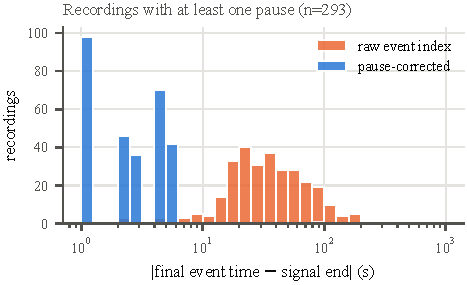
\includegraphics[width=\columnwidth]{figures/alignment.pdf}
\caption{Offset between the final \textit{Paused} event and the end of the EDF signal for recordings
containing pauses, before (orange) and after (blue) subtracting paused time. Offsets below 1\,s are
plotted at 1\,s.}
\label{fig:align}
\end{figure}

From the corrected events we build a per-second timeline with five states (eyes-closed, eyes-open,
photic, hyperventilation, unknown). Photic and hyperventilation override the eye state, and the 60\,s
after hyperventilation remain labelled hyperventilation. A per-second clean mask removes 1\,s before
and 3\,s after every state change (absorbing the residual offset), 3\,s around pause joins (filter
ringing at the discontinuity), 2\,s before to 3\,s after point artifacts (movement, coughing,
swallowing, talking, etc.), and 30\,s after drowsiness, sleep or snoring annotations.
Hyperventilation is labelled only so that it can be excluded: it is present in few recordings
(0.01--0.4 clean minutes on average per group) and induces EEG slowing in healthy subjects that would
mimic pathology, so it is used neither for segments nor for biomarkers.

\subsection{Age-normative clinical biomarkers}
\label{sec:bio}
For each recording we compute 48 biomarkers from Welch spectra of 4\,s windows (2\,s step, at most 150
windows per state):
\begin{itemize}
\item \textit{Eyes-closed (39):} log relative power in $\delta$ (1--4\,Hz), $\theta$ (4--8), $\alpha$
(8--13) and $\beta$ (13--30) for five regions; theta/alpha, delta/alpha and slow/fast ratios;
fronto-posterior alpha ratio; alpha and beta hemispheric asymmetry; posterior alpha centre of gravity
and peak frequency; spectral entropy; median frequency; total power; Hjorth mobility and complexity;
inter-hemispheric and fronto-posterior coherence in $\theta$, $\alpha$ and $\beta$.
\item \textit{Eyes-open (5):} global relative band powers and posterior alpha centre of gravity.
\item \textit{Reactivity and driving (2):} posterior \emph{alpha reactivity},
$\log(P_\alpha^{EC}/P_\alpha^{EO})$; and occipital \emph{photic-driving SNR}, the log ratio of O1/O2
power within $\pm0.5$\,Hz of the flash frequency to power 1--3\,Hz away, averaged over stimulation
blocks up to 25\,Hz.
\item \textit{Availability (2):} indicators \texttt{has\_eo} and \texttt{has\_photic}.
\end{itemize}
The set includes the eight clinical ratios used by CEFA-Net \cite{cefanet2026}. The reactivity and
photic-driving markers can only be computed with a correct event clock. Recording length is not an
input; each recording contributes a fixed number of segments.

Because EEG slows with healthy ageing, a raw biomarker confounds age with impairment. For every
biomarker $x_j$ we fit a linear age model on the \emph{training Normal recordings only} and replace
$x_j$ by its robust deviation
\begin{equation}
z_j = \frac{x_j - f_j(\text{age})}{1.4826\,\mathrm{MAD}_j},
\end{equation}
where $\mathrm{MAD}_j$ is the median absolute deviation of the normal residuals. Values are clipped to
$\pm6$; a missing state gives $z_j=0$ (typical for age), and the indicator records the absence. In
cross-validation the normative model is refitted within each fold.

\subsection{SANF-Net}
\label{sec:model}
SANF-Net (Fig.~\ref{fig:arch}) has three input branches.

\textbf{EEG branch.} A recording is a bag of 10\,s segments ($19 \times 1000$ samples) drawn from clean
seconds by state: 60\% eyes-closed, 25\% eyes-open and 15\% photic (12 segments per recording in
training, 24 at evaluation). A shared encoder applies three parallel temporal convolutions (0.11, 0.25
and 0.51\,s kernels, matching beta, alpha and delta--theta time scales), a depthwise spatial
convolution over the 19 channels, a separable convolution with squeeze-and-excitation (SE), a temporal
convolution with a second SE block, and mean and standard-deviation pooling to a 128-d embedding $h$.
Each embedding is modulated by its state $s$ with feature-wise linear modulation (FiLM)
\cite{perez2018film}, $h' = h\odot(1+\gamma_s)+\beta_s$, initialised to identity, and gated attention
pooling \cite{ilse2018attention} combines the segments of a recording.

\textbf{Biomarker and age branches.} The 48 normative $z$-scores pass through a two-layer MLP (64-d)
and standardised age through a small MLP (16-d). Age is an explicit input so that its contribution
can be measured and ablated.

\textbf{Modality-gated fusion.} Each branch is projected to 128-d; a linear layer over the
concatenated projections yields softmax gates $g\in\Delta^3$, and the fused vector is $\sum_m g_m h_m$.
The gates show how much each prediction relied on EEG, biomarkers or age. During training each
modality is dropped with probability 0.15 (never all at once), so that no single input, particularly
age, carries the model.

\textbf{Two heads.} Normal $<$ MCI $<$ Dementia is an ordered scale. Besides a softmax head, an ordinal
cumulative-link head \cite{mccullagh1980regression} predicts a severity score $s_{\mathrm{sev}}$ and two
ordered thresholds $t_1<t_2$, with $P(y>k)=\sigma(s_{\mathrm{sev}}-t_k)$. The class probabilities of
the two heads are averaged.

\begin{figure}[t]
\centering
\resizebox{\columnwidth}{!}{% SANF-Net architecture (TikZ). Included from main.tex with % SANF-Net architecture (TikZ). Included from main.tex with % SANF-Net architecture (TikZ). Included from main.tex with \input{figures/architecture}.
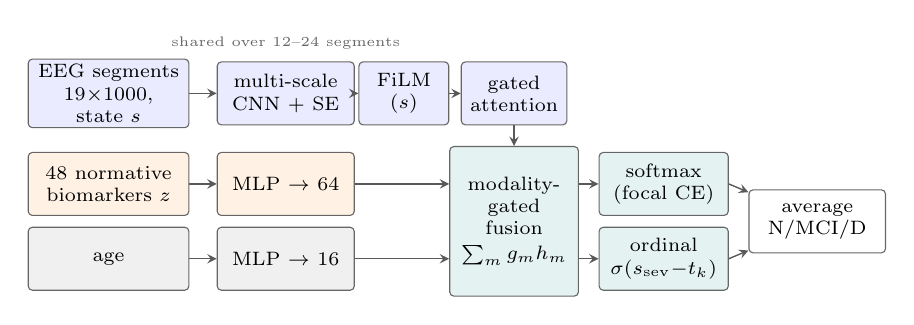
\begin{tikzpicture}[
  font=\scriptsize, >=stealth,
  blk/.style={draw=black!60, rounded corners=1.5pt, align=center, inner sep=2pt,
              minimum height=8mm, text width=#1},
  blk/.default=19mm,
  arr/.style={->, draw=black!65, line width=0.5pt}]
\def\ya{0} \def\yb{-1.15} \def\yc{-2.1}

% inputs
\node[blk, fill=blue!8]    (seg) at (0,\ya) {EEG segments\\$19{\times}1000$, state $s$};
\node[blk, fill=orange!10] (bm)  at (0,\yb) {48 normative\\biomarkers $z$};
\node[blk, fill=black!6]   (ag)  at (0,\yc) {age};

% branches
\node[blk=16mm, fill=blue!8]    (enc)  at (2.25,\ya) {multi-scale\\CNN + SE};
\node[blk=10mm, fill=blue!8]    (film) at (3.75,\ya) {FiLM\\($s$)};
\node[blk=12mm, fill=blue!8]    (pool) at (5.15,\ya) {gated\\attention};
\node[blk=16mm, fill=orange!10] (bmlp) at (2.25,\yb) {MLP $\to$ 64};
\node[blk=16mm, fill=black!6]   (amlp) at (2.25,\yc) {MLP $\to$ 16};

% fusion (spans the biomarker and age rows)
\node[draw=black!60, rounded corners=1.5pt, fill=teal!10, align=center, text width=14mm,
      minimum height=19mm] (fuse) at (5.15,{(\yb+\yc)/2}) {modality-\\gated\\fusion\\[1pt]$\sum_m g_m h_m$};

% heads and output
\node[blk=15mm, fill=teal!10] (soft) at (7.05,\yb) {softmax\\(focal CE)};
\node[blk=15mm, fill=teal!10] (ord)  at (7.05,\yc) {ordinal\\$\sigma(s_{\mathrm{sev}}{-}t_k)$};
\node[draw=black!60, rounded corners=1.5pt, align=center, text width=15mm, minimum height=8mm]
      (out) at (9.0,{(\yb+\yc)/2}) {average\\N/MCI/D};

\draw[arr] (seg) -- (enc);
\draw[arr] (enc) -- (film);
\draw[arr] (film) -- (pool);
\draw[arr] (pool) -- (fuse);
\draw[arr] (bm) -- (bmlp);
\draw[arr] (ag) -- (amlp);
\draw[arr] (bmlp) -- (bmlp -| fuse.west);
\draw[arr] (amlp) -- (amlp -| fuse.west);
\draw[arr] (fuse.east |- soft) -- (soft);
\draw[arr] (fuse.east |- ord) -- (ord);
\draw[arr] (soft.east) -- (out);
\draw[arr] (ord.east) -- (out);
\node[font=\tiny, color=black!60, above=0.3mm of enc] {shared over 12--24 segments};
\end{tikzpicture}
.
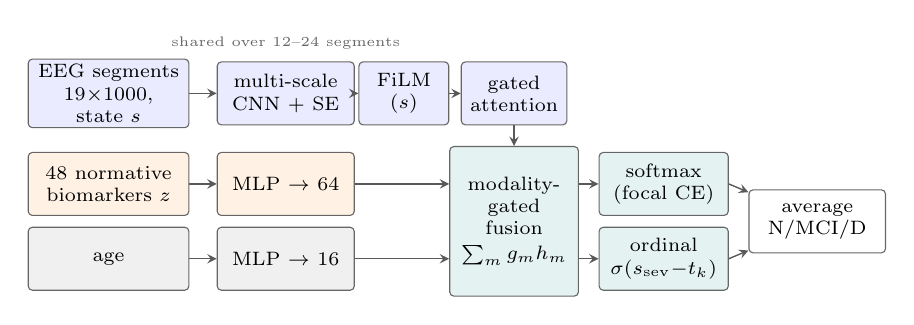
\begin{tikzpicture}[
  font=\scriptsize, >=stealth,
  blk/.style={draw=black!60, rounded corners=1.5pt, align=center, inner sep=2pt,
              minimum height=8mm, text width=#1},
  blk/.default=19mm,
  arr/.style={->, draw=black!65, line width=0.5pt}]
\def\ya{0} \def\yb{-1.15} \def\yc{-2.1}

% inputs
\node[blk, fill=blue!8]    (seg) at (0,\ya) {EEG segments\\$19{\times}1000$, state $s$};
\node[blk, fill=orange!10] (bm)  at (0,\yb) {48 normative\\biomarkers $z$};
\node[blk, fill=black!6]   (ag)  at (0,\yc) {age};

% branches
\node[blk=16mm, fill=blue!8]    (enc)  at (2.25,\ya) {multi-scale\\CNN + SE};
\node[blk=10mm, fill=blue!8]    (film) at (3.75,\ya) {FiLM\\($s$)};
\node[blk=12mm, fill=blue!8]    (pool) at (5.15,\ya) {gated\\attention};
\node[blk=16mm, fill=orange!10] (bmlp) at (2.25,\yb) {MLP $\to$ 64};
\node[blk=16mm, fill=black!6]   (amlp) at (2.25,\yc) {MLP $\to$ 16};

% fusion (spans the biomarker and age rows)
\node[draw=black!60, rounded corners=1.5pt, fill=teal!10, align=center, text width=14mm,
      minimum height=19mm] (fuse) at (5.15,{(\yb+\yc)/2}) {modality-\\gated\\fusion\\[1pt]$\sum_m g_m h_m$};

% heads and output
\node[blk=15mm, fill=teal!10] (soft) at (7.05,\yb) {softmax\\(focal CE)};
\node[blk=15mm, fill=teal!10] (ord)  at (7.05,\yc) {ordinal\\$\sigma(s_{\mathrm{sev}}{-}t_k)$};
\node[draw=black!60, rounded corners=1.5pt, align=center, text width=15mm, minimum height=8mm]
      (out) at (9.0,{(\yb+\yc)/2}) {average\\N/MCI/D};

\draw[arr] (seg) -- (enc);
\draw[arr] (enc) -- (film);
\draw[arr] (film) -- (pool);
\draw[arr] (pool) -- (fuse);
\draw[arr] (bm) -- (bmlp);
\draw[arr] (ag) -- (amlp);
\draw[arr] (bmlp) -- (bmlp -| fuse.west);
\draw[arr] (amlp) -- (amlp -| fuse.west);
\draw[arr] (fuse.east |- soft) -- (soft);
\draw[arr] (fuse.east |- ord) -- (ord);
\draw[arr] (soft.east) -- (out);
\draw[arr] (ord.east) -- (out);
\node[font=\tiny, color=black!60, above=0.3mm of enc] {shared over 12--24 segments};
\end{tikzpicture}
.
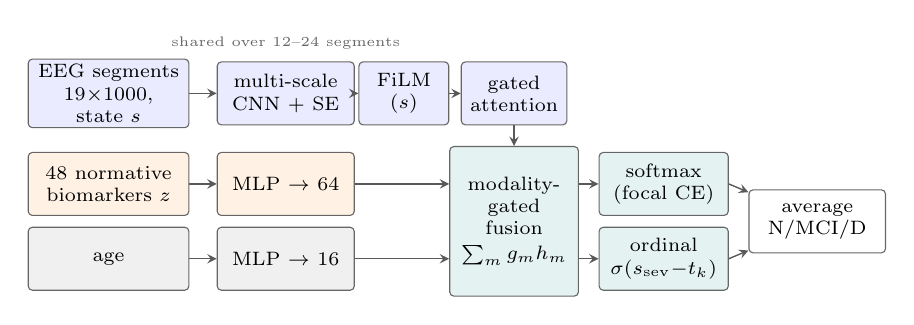
\begin{tikzpicture}[
  font=\scriptsize, >=stealth,
  blk/.style={draw=black!60, rounded corners=1.5pt, align=center, inner sep=2pt,
              minimum height=8mm, text width=#1},
  blk/.default=19mm,
  arr/.style={->, draw=black!65, line width=0.5pt}]
\def\ya{0} \def\yb{-1.15} \def\yc{-2.1}

% inputs
\node[blk, fill=blue!8]    (seg) at (0,\ya) {EEG segments\\$19{\times}1000$, state $s$};
\node[blk, fill=orange!10] (bm)  at (0,\yb) {48 normative\\biomarkers $z$};
\node[blk, fill=black!6]   (ag)  at (0,\yc) {age};

% branches
\node[blk=16mm, fill=blue!8]    (enc)  at (2.25,\ya) {multi-scale\\CNN + SE};
\node[blk=10mm, fill=blue!8]    (film) at (3.75,\ya) {FiLM\\($s$)};
\node[blk=12mm, fill=blue!8]    (pool) at (5.15,\ya) {gated\\attention};
\node[blk=16mm, fill=orange!10] (bmlp) at (2.25,\yb) {MLP $\to$ 64};
\node[blk=16mm, fill=black!6]   (amlp) at (2.25,\yc) {MLP $\to$ 16};

% fusion (spans the biomarker and age rows)
\node[draw=black!60, rounded corners=1.5pt, fill=teal!10, align=center, text width=14mm,
      minimum height=19mm] (fuse) at (5.15,{(\yb+\yc)/2}) {modality-\\gated\\fusion\\[1pt]$\sum_m g_m h_m$};

% heads and output
\node[blk=15mm, fill=teal!10] (soft) at (7.05,\yb) {softmax\\(focal CE)};
\node[blk=15mm, fill=teal!10] (ord)  at (7.05,\yc) {ordinal\\$\sigma(s_{\mathrm{sev}}{-}t_k)$};
\node[draw=black!60, rounded corners=1.5pt, align=center, text width=15mm, minimum height=8mm]
      (out) at (9.0,{(\yb+\yc)/2}) {average\\N/MCI/D};

\draw[arr] (seg) -- (enc);
\draw[arr] (enc) -- (film);
\draw[arr] (film) -- (pool);
\draw[arr] (pool) -- (fuse);
\draw[arr] (bm) -- (bmlp);
\draw[arr] (ag) -- (amlp);
\draw[arr] (bmlp) -- (bmlp -| fuse.west);
\draw[arr] (amlp) -- (amlp -| fuse.west);
\draw[arr] (fuse.east |- soft) -- (soft);
\draw[arr] (fuse.east |- ord) -- (ord);
\draw[arr] (soft.east) -- (out);
\draw[arr] (ord.east) -- (out);
\node[font=\tiny, color=black!60, above=0.3mm of enc] {shared over 12--24 segments};
\end{tikzpicture}
}
\caption{SANF-Net. State-tagged EEG segments, age-normative biomarkers and age are encoded separately
and combined by modality-gated fusion feeding a softmax and an ordinal head.}
\label{fig:arch}
\end{figure}

\subsection{Training}
The loss is a class-weighted focal cross-entropy \cite{lin2017focal} ($\gamma=1.5$, weights
1.0/1.4/1.2 for Normal/MCI/Dementia, label smoothing 0.05) plus 0.5 times the cumulative binary
cross-entropy of the ordinal head. We train for 35 epochs with AdamW (learning rate $10^{-3}$, weight
decay 0.05, 3-epoch warm-up then cosine decay), 16 recordings per batch, mixed precision, gradient
clipping at 2.0 and an exponential moving average (EMA) of the weights (decay 0.995). Augmentation
comprises amplitude scaling (0.9--1.1), Gaussian noise, channel dropout (0.1), biomarker noise and
\emph{same-class bag mixing}: with probability 0.3, 25--50\% of a recording's segments are replaced by
segments of another training recording with the same label. The network has 143k parameters and
trains in about 6\,min per fold on a laptop RTX~4050 GPU. We evaluate the final EMA weights rather than
selecting a checkpoint on a small validation set.

\subsection{Evaluation protocol}
All metrics are per recording. Our primary protocol is stratified five-fold cross-validation over the
pooled 1,069 training and validation recordings, with the normative model and age scaling refitted in
each fold, giving one out-of-fold (OOF) prediction per recording. The main models are evaluated with
five different fold assignments (repeated CV, $5\times5$) and reported as mean $\pm$ s.d.\ over repeats;
ablations and subgroup analyses use the first fold assignment. We also report the official test and
no-overlap test sets, scored by the mean prediction of the five fold models. Metrics are accuracy,
balanced accuracy, macro one-vs-rest AUC, per-class recall and pairwise AUCs, with 95\% percentile
bootstrap confidence intervals (1,000 resamples of recordings); model differences use a paired
bootstrap on the same OOF recordings. Subgroup counts in OOF analyses refer to the 1,069 pooled
recordings (229 community normals, 171 SMI).

\textbf{Baselines,} all with exactly the same folds and per-fold normative refitting.
\textit{Tabular:} age alone; the 48 biomarkers, raw or normative; normative biomarkers plus age; each
with $L_2$-regularised logistic regression (LR; class-balanced, $C$ tuned by inner five-fold CV) and,
for the last, histogram gradient boosting (HGB). \textit{Deep, EEG from random crops:} EEGNet-8,2
\cite{lawhern2018eegnet} and a CEEDNet-style 1D-ResNet (four stages of two residual blocks on the raw
19 channels, age concatenated before the classifier, 2.3M parameters) \cite{kim2023caueeg}. Both use
SANF-Net's data pipeline, loss, schedule, augmentation and EMA, and average segment logits per
recording; the 1D-ResNet follows CEEDNet's design idea but is not the authors' code or training
recipe.

% ============================================================================
\section{Results}
\label{sec:results}

\subsection{Main results}
Table~\ref{tab:main} summarises three-class performance. On the first fold assignment SANF-Net reaches
59.8\% OOF accuracy (95\% CI 56.7--62.8\%) and a macro AUC of 0.780 (0.759--0.801); over four repeated
fold assignments it reaches $59.5\pm0.3\%$ and $0.778\pm0.006$. On the official test split the five-fold ensemble scores 66.1\%
(57.6--74.6\%) with AUC 0.862, and 64.4\% (AUC 0.853) on the no-overlap subset. The test split is
easier than the pooled data: the same architecture trained on the official split scores
$59.9\pm1.0\%$ on validation but $68.4\pm2.8\%$ on test (3 seeds). Single-split numbers on CAUEEG
should therefore be read with intervals of about $\pm 8$ points.

The tabular baselines are strong. Age alone gives 51.1\% (AUC 0.709), and logistic regression on
normative biomarkers plus age reaches $59.3\pm0.7\%$ (AUC $0.778\pm0.004$) over five repeats. On the
first fold assignment the paired difference from SANF-Net is $+0.2$ points in accuracy (95\% CI $-2.7$
to $+3.3$) and $+0.003$ in AUC ($-0.013$ to $+0.020$); over the four shared fold assignments it is $-0.1\pm0.5$ points and $-0.001\pm0.006$ AUC: the two models are indistinguishable. The
deep EEG-only baselines are weaker: EEGNet reaches 52.9\% (AUC 0.707) and the 1D-ResNet 57.7\% (AUC 0.752).
SANF-Net is significantly better than EEGNet ($+6.8$ points, CI 3.4--10.1) and than the 1D-ResNet in
AUC ($+0.028$, CI 0.003--0.050), though not in accuracy ($+2.1$, CI $-1.4$ to $+5.4$). On the official
test split the 1D-ResNet scores 61.0\%, below the published 70.2\% for CEEDNet, which used a larger
model, longer training and test-time augmentation; we do not claim to reproduce it.

\begin{table}[t]
\centering
\caption{Three-class results (per recording). CV: 5-fold out-of-fold, $n=1069$ (mean $\pm$ s.d.\
over 5 fold assignments where marked $^\ast$; 4 for SANF-Net). Test: official test split, $n=118$, mean of the five
fold models of the first assignment.}
\label{tab:main}
\resizebox{\columnwidth}{!}{%
\begin{tabular}{lcccccc}
\toprule
& \multicolumn{3}{c}{CV out-of-fold} & \multicolumn{3}{c}{Test}\\
\cmidrule(lr){2-4}\cmidrule(lr){5-7}
Model & Acc & BAcc & AUC & Acc & BAcc & AUC\\
\midrule
Age (LR)$^\ast$ & $51.1\pm0.2$ & $51.6\pm0.2$ & $.709\pm.002$ & 55.1 & 54.6 & .739\\
Biomarkers, raw (LR) & 56.0 & 56.0 & .761 & 63.6 & 63.5 & .815\\
Biomarkers, normative (LR) & 58.1 & 58.1 & .761 & 62.7 & 63.2 & .809\\
Norm.\ biomarkers + age (LR)$^\ast$ & $59.3\pm0.7$ & $59.3\pm0.7$ & $.778\pm.004$ & 66.1 & 65.9 & .839\\
Norm.\ biomarkers + age (HGB) & 59.2 & 58.9 & .779 & 61.0 & 60.2 & .813\\
EEGNet \cite{lawhern2018eegnet} & 52.9 & 51.5 & .707 & 60.2 & 58.0 & .773\\
1D-ResNet (CEEDNet-style) & 57.7 & 57.1 & .752 & 61.0 & 60.0 & .810\\
CEEDNet \cite{kim2023caueeg}$^\dagger$ & -- & -- & -- & 70.2 & -- & --\\
\midrule
SANF-Net (ours)$^\ast$ & $59.5\pm0.3$ & $59.1\pm0.4$ & $.778\pm.006$ & 66.1 & 66.1 & .862\\
\bottomrule
\multicolumn{7}{l}{\footnotesize $^\dagger$As published (own training recipe and test-time
augmentation); 74.7\% with a 9-model ensemble.}
\end{tabular}}
\end{table}

\begin{figure}[t]
\centering
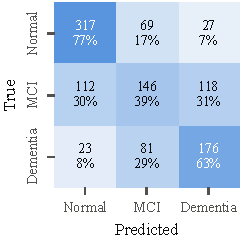
\includegraphics[width=0.62\columnwidth]{figures/confusion.pdf}
\caption{SANF-Net out-of-fold confusion matrix ($n=1069$, first fold assignment; counts and row
percentages).}
\label{fig:cm}
\end{figure}

\textbf{MCI is the bottleneck.} Recall is 76.8\% for Normal, 62.9\% for Dementia and only 38.8\%
(33.9--44.1\%) for MCI, whose errors split evenly between Normal and Dementia (Fig.~\ref{fig:cm}). For
MCI versus Normal, SANF-Net's AUC is 0.787 (0.752--0.818), detecting 63\% of MCI at 80\% specificity.
Here the linear model is significantly better (AUC 0.823; paired difference $-0.037$, CI $-0.057$ to
$-0.018$; Fig.~\ref{fig:roc}, left), and it also has higher MCI recall (47.9\% versus 38.8\%). Age alone
already achieves 0.754. Section~\ref{sec:confound} shows that the linear model's advantage comes from
the protocol features.

\subsection{Ablations}
\label{sec:ablation}
Table~\ref{tab:ablation} removes one component of SANF-Net at a time under the same protocol (first
fold assignment); paired bootstrap CIs are relative to the full model. Only removing both
non-EEG branches clearly hurts: the EEG-only network loses 4.5 accuracy points (CI 1.4--8.0), 0.049
macro AUC and 0.068 MCI-versus-Normal AUC, and its MCI recall falls to 24.5\%. Every single
component is worth at most about two accuracy points, and no single removal is significant in
accuracy. State-aware cropping gives a small but significant AUC gain ($+0.013$, CI 0.002--0.025);
normative scoring ($+0.018$) and the biomarker branch ($+0.020$) help MCI-versus-Normal AUC with CIs
just touching zero. FiLM, attention pooling and the age input are not distinguishable from zero.
Removing the ordinal head leaves accuracy and AUC unchanged but moves the operating point: MCI recall
rises from 38.8\% to 58.8\%, at the cost of Normal (76.8 to 68.3\%) and Dementia (62.9 to 47.5\%)
recall. The ordinal loss therefore pulls borderline cases towards the extreme classes rather than
adding information.

\begin{table}[t]
\centering
\caption{Ablations (5-fold CV out-of-fold, $n=1069$, first fold assignment).}
\label{tab:ablation}
\resizebox{\columnwidth}{!}{%
\begin{tabular}{lcccc}
\toprule
Variant & Acc & AUC & \shortstack{AUC\\N vs MCI} & \shortstack{MCI\\recall}\\
\midrule
SANF-Net (full) & 59.8 & .780 & .787 & 38.8\\
\quad random crops, no state & 58.6 & .767 & .781 & 36.2\\
\quad no FiLM state conditioning & 58.9 & .777 & .784 & 41.8\\
\quad mean instead of attention pool & 58.5 & .782 & .783 & 35.9\\
\quad plain standardisation (no normative) & 57.6 & .768 & .768 & 36.4\\
\quad no biomarkers & 57.3 & .772 & .767 & 34.8\\
\quad no age & 58.5 & .783 & .788 & 37.0\\
\quad EEG only & 55.3 & .731 & .719 & 24.5\\
\quad no ordinal head & 59.5 & .777 & .785 & 58.8\\
\bottomrule
\end{tabular}}
\end{table}

\subsection{Protocol and age confounds}
\label{sec:confound}
Community-recruited normals differ from every other group in ways unrelated to cognition
(Table~\ref{tab:groups}, Fig.~\ref{fig:protocol}). They are younger (61.7 versus 69.6--76.6 years),
only 12\% of their recordings include photic stimulation (versus 90\% of SMI, 92\% of MCI and 92\% of
dementia recordings), fewer include an eyes-open period (63\% versus 80--87\%), and their recordings
are shorter (10.2 versus 13.8--14.0\,min). A model can therefore recognise many community normals from
the protocol alone: the \texttt{has\_photic} and \texttt{has\_eo} indicators, the photic-driving
feature, and the presence of photic segments in the EEG bag all encode it.

\begin{figure}[t]
\centering
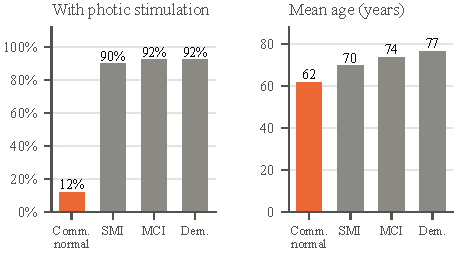
\includegraphics[width=\columnwidth]{figures/protocol.pdf}
\caption{Share of recordings with photic stimulation and mean age per subgroup. Community normals
(orange) differ from all clinical groups in both, independently of cognition.}
\label{fig:protocol}
\end{figure}

\textbf{Protocol-blind models.} We trained (A) SANF-Net with photic segments removed from the EEG bag
and \texttt{has\_photic}, \texttt{has\_eo} and photic-driving SNR removed from the biomarkers;
(B) SANF-Net on eyes-closed segments only, which also removes eyes-open availability from the EEG
branch; and the linear model without the same three features. Table~\ref{tab:confound} shows that
every model separates community normals from MCI far better than SMI patients from MCI. Removing
protocol information costs SANF-Net 2.7 accuracy points (CI $+0.1$ to $+5.1$) and 0.016 AUC
(0.002--0.030), and costs the linear model $2.5$ points and 0.031 AUC (means over five repeats). The
loss falls almost entirely on the community-versus-MCI comparison (0.891$\to$0.852 for SANF-Net,
0.951$\to$0.863 for LR), whereas SMI-versus-MCI stays at 0.65--0.66 for every model. Without protocol
features the linear model's MCI-versus-Normal advantage disappears: its AUC falls from 0.822 to 0.775,
against 0.764 for protocol-blind SANF-Net.

\begin{table}[t]
\centering
\caption{Protocol confound (5-fold CV out-of-fold, $n=1069$). Comm.: community-recruited normals
($n=229$); SMI: subjective memory impairment ($n=171$). LR rows: mean over 5 fold assignments.}
\label{tab:confound}
\resizebox{\columnwidth}{!}{%
\begin{tabular}{lccccc}
\toprule
& & & \multicolumn{2}{c}{AUC vs MCI} & \\
\cmidrule(lr){4-5}
Model & Acc & AUC & Comm. & SMI & \shortstack{SMI\\recall}\\
\midrule
Age (LR) & 51.1 & .709 & .858 & .618 & 42.7\\
Norm.\ biomarkers + age (LR) & 59.3 & .778 & .951 & .655 & 35.7\\
\quad without protocol features & 56.8 & .747 & .863 & .660 & 50.6\\
SANF-Net & 59.8 & .780 & .891 & .653 & 57.9\\
\quad (A) no photic information & 57.1 & .764 & .852 & .649 & 63.7\\
\quad (B) eyes-closed only & 58.5 & .756 & .842 & .650 & 63.7\\
\bottomrule
\end{tabular}}
\end{table}

\textbf{Age-matched analysis.} Age and protocol are entangled, because community normals are both
younger and differently recorded. We therefore matched each comparison group 1:1 to MCI recordings by
age (greedy nearest neighbour without replacement, caliper 2 years) on the OOF predictions and
recomputed AUCs (Table~\ref{tab:matched}); an age-only model scores 0.50--0.51 on every matched set,
confirming the matching. With age removed, the linear model still separates community normals from
MCI (0.864), but almost entirely through protocol: without protocol features it drops to 0.615, and
protocol-blind SANF-Net (A) to 0.570. On the 24 community normals whose recording \emph{did} include
photic stimulation, matched to MCI with the same protocol, no model exceeds chance (0.50--0.59, all
CIs include 0.5). SMI versus age-matched MCI, where protocol is shared, gives 0.54--0.57 for every
model.

\begin{table}[t]
\centering
\caption{Age-matched AUC versus MCI (1:1, caliper 2 years) on out-of-fold predictions, with 95\%
bootstrap CI over matched pairs.}
\label{tab:matched}
\resizebox{\columnwidth}{!}{%
\begin{tabular}{lcccc}
\toprule
& Community & \shortstack{Community\\with photic} & SMI\\
\midrule
Matched pairs & 127 & 24 & 168\\
Mean age (group / MCI) & 66.2 / 66.5 & 63.9 / 63.8 & 70.5 / 70.6\\
\midrule
Age (LR) & .51 (.50--.52) & .50 (.47--.53) & .50 (.49--.50)\\
Norm.\ biomarkers + age (LR) & .86 (.82--.91) & .56 (.45--.69) & .57 (.52--.62)\\
\quad without protocol features & .62 (.57--.66) & .59 (.48--.71) & .55 (.51--.59)\\
SANF-Net & .71 (.66--.77) & .50 (.37--.62) & .54 (.50--.58)\\
\quad (A) no photic information & .57 (.53--.61) & .52 (.40--.65) & .54 (.51--.58)\\
\bottomrule
\end{tabular}}
\end{table}

\subsection{What the model uses}
The mean modality gates differ by true class: for Normal recordings the EEG branch dominates (EEG 0.42,
biomarkers 0.29, age 0.29), whereas for MCI and Dementia the biomarker branch dominates (0.40 and 0.42)
and EEG falls to 0.28--0.30. Given Table~\ref{tab:matched}, the EEG branch's weight on Normal
recordings is consistent with it detecting the absence of photic segments rather than normal
physiology.

\textbf{A cautionary note on development.} SANF-Net's design was developed on the official split, and
the official test set was consulted during development. In particular, we screened additional feature
families (aperiodic exponent, permutation entropy and Lempel--Ziv complexity, wPLI and
amplitude-envelope connectivity, band-power variability, microstates); adding connectivity improved
the official test accuracy (73.7\% versus 72.9\% for a single model) but gave no gain under five-fold
CV (59.3\% versus 59.8\%), and we did not adopt it. Official-test numbers for SANF-Net are therefore
not strictly held out, which is one reason we treat cross-validated OOF results as primary.

\subsection{External validation}
\label{sec:external}
Table~\ref{tab:external} and Fig.~\ref{fig:roc} (right) report MCI-versus-normal performance without
retraining, using the same five fold models as all CAUEEG results (each paired with its own fold's
normative model, predictions averaged). Since age is uninformative here, these results reflect EEG and
biomarkers only. We also apply a label-free \emph{site calibration}: channel amplitudes are rescaled to
the external cohort's median, and normative $z$-scores are re-centred and re-scaled on the cohort's own
normals in a leave-one-out manner, so no subject contributes to its own reference. On the pooled Isfahan cohorts the
CV ensemble reaches an AUC of 0.67 (0.53--0.80), rising to 0.70 with site calibration; on GENEEG it is
0.58 (0.44--0.72) with or without calibration, an interval that includes chance. With 61--63 subjects per cohort all intervals are wide. The
models trained on the official split (3 seeds) gave similar results (Isfahan pooled 0.649, 0.677 with
calibration; GENEEG 0.560, 0.563).

\begin{table}[t]
\centering
\caption{External MCI vs.\ normal without retraining (5-fold CV ensemble). AUC with 95\% bootstrap
CI.}
\label{tab:external}
\resizebox{\columnwidth}{!}{%
\begin{tabular}{lccc}
\toprule
Cohort & $n$ (MCI) & No calibration & Site calibration\\
\midrule
Isfahan 2016 & 27 (11) & .73 (.51--.91) & .76 (.57--.92)\\
Isfahan 2019 & 34 (18) & .64 (.45--.84) & .63 (.44--.81)\\
Isfahan pooled & 61 (29) & .67 (.53--.80) & .70 (.56--.83)\\
GENEEG & 63 (28) & .58 (.44--.72) & .58 (.42--.74)\\
\bottomrule
\end{tabular}}
\end{table}

\begin{figure}[t]
\centering
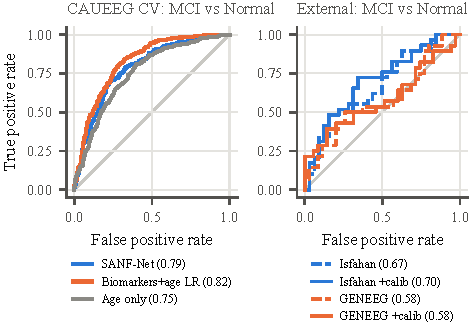
\includegraphics[width=\columnwidth]{figures/roc.pdf}
\caption{MCI versus normal ROC curves. Left: CAUEEG five-fold out-of-fold predictions (AUC in
brackets). Right: external cohorts without retraining, with and without site calibration.}
\label{fig:roc}
\end{figure}

% ============================================================================
\section{Discussion}

\textbf{Much of the MCI signal is age and protocol.} The headline MCI-versus-Normal AUCs on CAUEEG
(0.70--0.82 for every model here) mix three sources: age, recording protocol and EEG physiology. Age
alone gives 0.75. After age matching, the clinically relevant comparison, a patient with memory
complaints who does or does not have MCI, reaches only 0.54--0.57, and community normals recorded with
the same protocol as MCI patients are not distinguished from them. This agrees with Mishra
\textit{et al.}'s observation of strongly overlapping MCI and control EEG feature distributions
\cite{geneeg2025}, and suggests a low ceiling for resting-state spectral EEG as an MCI screen. We
recommend that CAUEEG results be reported per Normal subgroup, with age-matched comparisons.

\textbf{The linear model's MCI advantage is a shortcut.} The linear model is significantly better than
SANF-Net for MCI versus Normal (0.823 versus 0.787) and recalls more MCI. Tables~\ref{tab:confound}
and~\ref{tab:matched} show where this comes from: given the protocol indicators, a linear model can
identify community normals almost perfectly (age-matched AUC 0.86, 0.90 for those without photic
stimulation), which leaves its Normal-versus-MCI boundary free to classify more borderline cases as
MCI. Once protocol features are removed, the advantage disappears (0.775 versus 0.764 for
protocol-blind SANF-Net). SANF-Net is less dependent on the shortcut, as its higher SMI recall shows
(57.9\% versus 35.7\%).

\textbf{Architecture versus features.} SANF-Net matches but does not beat logistic regression on the same
normative biomarkers. It beats the EEG-only deep baselines mainly because it also sees those
biomarkers and age: its own EEG-only ablation (55.3\%, AUC 0.731) lies between EEGNet and the 1D-ResNet. Gains in the deep-learning literature on
this benchmark should therefore be compared against a strong tabular model of established markers and
age under the same protocol; without that comparison, gains from architecture cannot be separated from
gains from features, age and protocol.

\textbf{Shortcuts need events to be seen.} The protocol confound is invisible to pipelines that take
random crops and ignore annotations, yet such models can still exploit it, because photic driving is
visible in the raw EEG. Correcting the event clock was a prerequisite both for the state-aware model
and for detecting the confound.

\textbf{Single splits mislead.} The official test split is easier than the pooled data by about 8 points,
and a feature family that improved the test score showed no gain under cross-validation.
Cross-validated OOF estimates with intervals and repeated fold assignments should be the primary
CAUEEG metric.

\textbf{Transfer.} Without retraining or age information, the CAUEEG models keep modest MCI
discrimination on Isfahan (AUC 0.67--0.70) but little on GENEEG (0.58), whose recordings differ more
in montage and protocol.
Re-centring normative references on a site's own normals is cheap and label-free, but the external
cohorts are too small for firm conclusions.

\textbf{Limitations.} Training data come from a single hospital. Subgroup labels rely on the dataset's
symptom codes, and the community-with-photic subgroup is small (24 matched pairs). The external
cohorts are small, lack ages and state annotations, and were not recorded with the CAUEEG protocol.
Diagnoses are clinical, without biomarker confirmation. The official test set was consulted during
model development. Ablations and subgroup analyses use a single fold assignment.

% ============================================================================
\section{Conclusion}
CAUEEG event annotations need a pause correction before they can be used. Once corrected, they enable
state-aware, age-normative modelling of MCI and dementia, and they reveal that community-recruited
normals are distinguishable by recording protocol and age alone. SANF-Net, a compact fusion network
built on these ideas, reaches 59.5\% repeated-CV accuracy and is less dependent on the protocol
shortcut than a tabular model, but does not outperform a linear model of normative biomarkers. Once age
and protocol are controlled, no model separates SMI or protocol-matched normals from MCI with an AUC
above 0.6. We release our event-alignment code and evaluation protocol \todo{repository URL} to
support confound-aware benchmarking of EEG-based cognitive screening.

% ============================================================================
\section*{Acknowledgment}
We thank the creators of CAUEEG, the Isfahan MCI datasets and GENEEG for making their data available.
\todo{Funding / institutional acknowledgements.}

\bibliographystyle{IEEEtran}
\bibliography{references}

\end{document}
